\documentclass[compress]{beamer}        % [compress] (written before {beamer} <=> navigation bar one line, all subsections in 1 line instead of 2

% Setup appearance:
\usetheme{CambridgeUS}
%	AnnArbor | Antibes | Bergen |
%	Berkeley | Berlin | Boadilla |
%	boxes | CambridgeUS | Copenhagen |
%	Darmstadt | default | Dresden |
%	Frankfurt | Goettingen |Hannover |
%	Ilmenau | JuanLesPins | Luebeck |
%	Madrid | Malmoe | Marburg |
%	Montpellier | PaloAlto | Pittsburgh |
%	Rochester | Singapore | Szeged |
%	Warsaw
%

\useoutertheme[footline=authorinstitute,subsection=false]{miniframes}
\usecolortheme{whale}

%	albatross | beaver | beetle |
%	crane | default | dolphin |
%	dove | fly | lily | orchid |
%	rose |seagull | seahorse |
%	sidebartab | structure |
%	whale | wolverine


\setbeamertemplate{footline}
{
  \hbox{%
  \begin{beamercolorbox}[wd=.25\paperwidth,ht=2.25ex,dp=1ex,center]{title in head/foot}%
    \usebeamerfont{date in head/foot}\insertshortauthor
  \end{beamercolorbox}%
  \begin{beamercolorbox}[wd=.5\paperwidth,ht=2.25ex,dp=1ex,center]{date in head/foot}%
    \usebeamerfont{title in head/foot}\insertshortinstitute
  \end{beamercolorbox}%
  \begin{beamercolorbox}[wd=.25\paperwidth,ht=2.25ex,dp=1ex,center]{title in head/foot}%
    \usebeamerfont{date in head/foot}
    \insertframenumber{} / \inserttotalframenumber
    %\insertframenumber{} / \insertpresentationendpage
  \end{beamercolorbox}}%
  \vskip0pt%
}

%\setbeamercolor{titlelike}{parent=structure}
%\setbeamercolor{structure}{fg=beamer@blendedblue}
%% \useinnertheme{rounded}
%\setbeamerfont{block title}{size={}}
%\usefonttheme[onlylarge]{structurebold}   % title and words in the table of contents bold
%\setbeamerfont*{frametitle}{size=\normalsize,series=\bfseries}
\setbeamertemplate{navigation symbols}{}
\setbeamercolor{frametitle}{parent=boxes, bg=white}
{ % only on titlepage


\usepackage{times}
\usepackage{amsmath,amssymb,amsthm}
\usepackage{color}
\usepackage{changepage}
\usepackage{multirow}
\usepackage[absolute,overlay]{textpos}
\usepackage{enumerate}
%\usepackage{pgfpages}
\usepackage[all]{xy}
\usepackage{textcomp}
\usepackage{etex}
\usepackage{tikz}
\usetikzlibrary{shapes}
%\usepackage{handoutWithNotes}
%\pgfpagesuselayout{4 on 1}[border shrink=1mm]




\definecolor{camblue}{RGB}{26,26,89}
\definecolor{Rblue}{RGB}{0,255,255}
\definecolor{Rdarkblue}{RGB}{0,0,255}
\definecolor{Rgreen}{RGB}{0,205,0}
\definecolor{green2}{RGB}{51,204,51}
\newcommand{\tcb}{\textcolor{beamer@blendedblue}}
\newcommand{\tcbb}{\textcolor{camblue}}
\newcommand{\tcr}{\textcolor{red}}
\newcommand{\tcg}{\textcolor{gray}}
\newcommand{\tcgr}{\textcolor{green2}}
\newcommand{\tcblk}{\textcolor{black}}
\newcommand{\tcRg}{\textcolor{Rgreen}}
\newcommand{\tcRdb}{\textcolor{Rdarkblue}}
\newcommand{\tcRb}{\textcolor{Rblue}}
\newcommand{\tcw}{\textcolor{white}}
\newcommand{\m}{\phantom{-}}
\newcommand{\bp}{\tcbb{$\bullet$}\:}


\title{{\huge Statistics for Computing\\[0.1cm]MA4413}}
\author[Kevin Burke]{{\bf\\[0.5cm]{\huge Lecture 13}\\[0.2cm]\emph{Statistical Estimation: Confidence Intervals}\\[1.4cm]Kevin Burke}\\[0.3cm]\tcb{kevin.burke@ul.ie}}

\institute[University of Limerick, Maths \& Stats Dept]{}
\date{}

%\TPGrid[5mm,5mm]{1}{1}

\begin{document}


\begin{frame}[t]
\titlepage
\end{frame}



\section{Return to Statistics}
\subsection{Statistics Recap}
\begin{frame}{\bf \tcb{Statistics Recap\\[-0.9cm]}}

\begin{itemize}\itemsep0.5cm
\item {\bf Population}: \emph{all} individuals / units of interest.
\item {\bf Parameter}: the particular \emph{feature} of the population that we are interested in.
\begin{itemize}\itemsep0.2cm
\item {\bf Mean}: $\mu =$ unknown (\emph{numeric} data).
\item {\bf Proportion}: $p =$ unknown (\emph{categorical} data).
\end{itemize}
\item {\bf Sample}: a set of $n$ individuals, selected via \emph{random sampling}, which informs us about the population.
\item {\bf Statistic}: the feature of interest calculated for the sample of data.
\begin{itemize}\itemsep0.2cm
\item {\bf Sample Mean}: $\bar x$ provides an estimate of $\mu$.
\item {\bf Sample Proportion}: $\hat p$ provides an estimate of $p$.\\[0.4cm]
\end{itemize}
\end{itemize}

Note that for numeric data we also have the \emph{population standard deviation}, $\sigma$, and the \emph{sample standard deviation}, $s$.

\end{frame}


\subsection{Diagrammatic Explanation}
\begin{frame}{\bf \tcb{Diagrammatic Explanation}}
\begin{displaymath}
\xymatrixcolsep{1.5cm}
\xymatrixrowsep{2cm}
    \xymatrix{
    \boxed{\text{\Huge Population}} \ar@{->}[r] \ar@/_2.2pc/[d]\ar@/_1.5pc/[d]\ar@/_0.8pc/[d]\ar@{->}[d]\ar@/^0.8pc/@{->}[d]\ar@/^1.5pc/@{->}[d]\ar@/^2.2pc/[d] &
    \begin{tikzpicture}[baseline=(char.base)]
      \node(char)[draw,shape=ellipse]{Parameter};
    \end{tikzpicture} \\
        \boxed{\text{Sample}} \ar@{->}[r] &
    \begin{tikzpicture}[baseline=(char.base)]
      \node(char)[draw,shape=ellipse]{Statistic};
    \end{tikzpicture} \ar@{.>}[u]}
\end{displaymath}

\begin{textblock}{1}(2.1,3.8)
\xymatrixrowsep{1cm}
\xymatrix{\\\ar@/^1.5pc/@{.}[u]}
\end{textblock}
\begin{textblock}{6}(2.2,3.3)
{\footnotesize\emph{\emph{All} individuals / units of interest}}
\end{textblock}

\begin{textblock}{1}(2.7,11.4)
\xymatrixrowsep{0.7cm}
\xymatrix{&\ar@/_1pc/@{.}[ld]\\&}
\end{textblock}
\begin{textblock}{5.5}(0.5,13)
{\footnotesize\emph{A subset of $n$ individuals}}
\end{textblock}

\begin{textblock}{1}(1.9,10)
\xymatrixcolsep{1.4cm}
\xymatrix{&\ar@/^0.5pc/@{.}[l]}
\end{textblock}
\begin{textblock}{3.5}(0.3,7.5)
{\footnotesize\emph{Select a representative sample via random sampling}}
\end{textblock}

\begin{textblock}{1}(13.4,3.8)
\xymatrixrowsep{1.3cm}
\xymatrix{\\\ar@/_1.5pc/@{.}[u]}
\end{textblock}
\begin{textblock}{5}(11,1.7)
{\footnotesize\emph{The true value (unknown):\\
Numeric data $\Rightarrow$ $\mu$\\
Categorical data $\Rightarrow$ $p$}}
\end{textblock}

\begin{textblock}{1}(13,11.4)
\xymatrixrowsep{1.2cm}
\xymatrix{\\\ar@/_1.8pc/@{.}[u]}
\end{textblock}
\begin{textblock}{6}(7.5,13)
{\footnotesize\emph{Estimated value (from sample):\\
Numeric data $\Rightarrow$ $\bar x$\\
Categorical data $\Rightarrow$ $\hat p$}}
\end{textblock}

\begin{textblock}{1}(11.8,7)
\xymatrixcolsep{0.7cm}
\xymatrix{\\&\ar@/_0.4pc/@{.}[l]}
\end{textblock}
\begin{textblock}{3}(13.2,7.5)
{\footnotesize\emph{An unbiased statistic estimates the parameter}}
\end{textblock}
\end{frame}


\subsection{Example: Android Application}
\begin{frame}{\bf \tcb{Example: Android Application\\[-0.9cm]}}

Developers of an Android application wish to know the average age of their users for the purposes of advertising. They contact $100$ users (selected via random sampling) and enquire about their age. Of these $100$ users, $68$ respond; the average age is found to be $22.54$ in this sample.\\[0.2cm]

\begin{itemize}\itemsep0.4cm
\item {\bf Population}: \emph{all} users.
\item {\bf Parameter}: The true mean age of all users; $\mu =$ unknown (must be estimated).
\item {\bf Sample}: The $n = 68$ users whose information we have.
\item {\bf Statistic}: The statistic is $\bar x = 22.54$ calculated based on our sample of $68$ users. This is used as an estimate of $\mu$.
\end{itemize}

\end{frame}



\subsection{Point Estimate Vs Interval Estimate}
\begin{frame}{\bf \tcb{Point Estimate Vs Interval Estimate}}

In the example just covered, the sample mean $\bar x = 22.54$ provides a {\bf point estimate} for the true population mean $\mu$.\\[0.6cm]

However, an {\bf interval estimate} is more useful, i.e., a \emph{range} of plausible values for $\mu$ based on the sample.\\[0.6cm]

For example, a statement such as ``we are 95\% confident that $\mu$ is contained in the interval $[21.83,\,23.25]$'' is much more useful than a single point estimate.\\[0.6cm]

Interval estimates take statistical variation into account and allow us to \emph{test hypotheses} about the true value $\mu$.

\end{frame}



\section{95\% Confidence Intervals}
\subsection{The Central Limit Theorem}
\begin{frame}{\bf \tcb{The Central Limit Theorem}}

The \emph{central limit theorem} tells us that

\begin{align*}
\,\overline{\!X} \sim \text{Normal}\left(\mu, \frac{\sigma}{\sqrt{n}}\right).\\
\end{align*}

Based on this fact, we know that 95\% of $\bar x$ values (calculated using different samples) would lie in the range $\mu \pm 1.96\,\frac{\sigma}{\sqrt{n}}$.\\[0.8cm]

Mathematical notation: $\Pr\left(\mu-1.96\,\frac{\sigma}{\sqrt{n}} < \,\overline{\!X} < \mu+1.96\,\frac{\sigma}{\sqrt{n}}\right) = 0.95$.\\[0.8cm]

{\footnotesize(note: we usually only have \emph{one} sample in practice, but the above result allows us to develop further theory)}

\end{frame}


\subsection{Manipulating the 95\% Limits}
\begin{frame}{\bf \tcb{Manipulating the 95\% Limits}}\label{maniplims}

In 95\% of samples $\,\overline{\!X} \in [\mu-1.96\,\frac{\sigma}{\sqrt{n}},\,\mu+1.96\,\frac{\sigma}{\sqrt{n}}]$,\\[0.2cm]
i.e., $\,\overline{\!X}$ is within $\pm 1.96\,\frac{\sigma}{\sqrt{n}}$ units of $\mu$.\\[1.2cm]

If $\,\overline{\!X}$ is within $\pm 1.96\,\frac{\sigma}{\sqrt{n}}$ units of $\mu$, then it is also true to say\\[0.2cm]that $\mu$ is within $\pm 1.96\,\frac{\sigma}{\sqrt{n}}$ units of $\,\overline{\!X}$.\\[1.2cm]
$\Rightarrow$ 95\% of the time $\mu \in [\,\overline{\!X}-1.96\,\frac{\sigma}{\sqrt{n}},\,\,\overline{\!X}+1.96\,\frac{\sigma}{\sqrt{n}}]$.\\[0.5cm]

\end{frame}



\subsection{95\% Confidence Interval}
\begin{frame}{\bf \tcb{95\% Confidence Interval}}

The interval $\,\overline{\!X}\pm1.96\,\frac{\sigma}{\sqrt{n}}$ is \emph{random}, i.e., it varies from sample to sample (since $\,\overline{\!X}$ varies).\\[0.6cm]

Typically we have \emph{one} sample of data and, hence, a specific sample mean value, $\bar x$. The calculated interval\\
\begin{align*}
\boxed{\bar x \pm1.96\,\frac{\sigma}{\sqrt{n}}}\\
\end{align*}
is called a {\bf 95\% confidence interval}.\\[0.6cm]


{\footnotesize(note: if we had multiple samples of data, the true mean, $\mu$, will be contained in 95\% of the calculated intervals)}
\end{frame}



\subsection{95\% Confidence Intervals: Multiple Samples}
\begin{frame}{\bf \tcb{95\% Confidence Intervals: Multiple Samples}\\[-1.1cm]}

\begin{center}
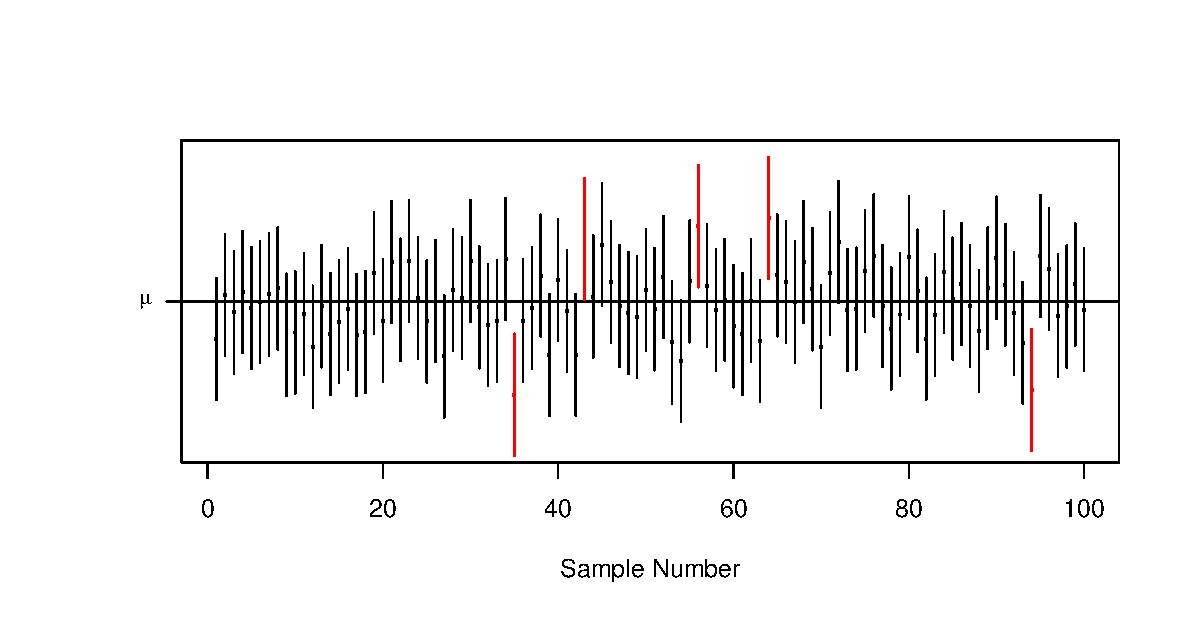
\includegraphics[width=1\textwidth, trim = 0.5cm 0.5cm 1cm 1.3cm, clip]{CIs}
\end{center}

\begin{itemize}
\item Sample means, $\bar x$, (dots) and 95\% confidence intervals, $\bar x \pm 1.96 \frac{\sigma}{\sqrt{n}}$, (vertical lines) calculated in multiple samples. Those which do not include $\mu$ are highlighted in red.
\end{itemize}


\end{frame}



\subsection{95\% Confidence Intervals: Multiple Samples}
\begin{frame}{\bf \tcb{95\% Confidence Intervals: Multiple Samples}\\[-1.1cm]}

\begin{center}
\includegraphics[width=1\textwidth, trim = 0.5cm 0.5cm 1cm 1.3cm, clip]{CIsLimits}
\end{center}

\begin{itemize}
\item 95\% limits around $\mu$ also shown. Note that if $\bar x \in \mu \pm 1.96 \frac{\sigma}{\sqrt{n}}$, then $\mu \in \bar x \pm 1.96 \frac{\sigma}{\sqrt{n}}$. In other words, $\mu$ and $\bar x$ are within $\pm1.96\frac{\sigma}{\sqrt{n}}$ units of each other in these cases (as developed in slide \pageref{maniplims}).
\end{itemize}


\end{frame}



\subsection{Terminology}
\begin{frame}{\bf \tcb{Terminology}}

Once a confidence interval is calculated, the phrase used is:\\[0.1cm]
{\bf``We are 95\% confident that {\boldmath$\mu$} is contained in this interval''}.\\[1cm]


Example:\\[0.2cm]
Let's assume $[21.83,\,23.25]$ is a 95\% confidence interval for $\mu$ calculated using a sample of data.\\[0.3cm]
Note that $\mu$ is a constant - \emph{it does not vary}. Therefore, it is either in the calculated interval or it is not.\\[0.3cm]
However, from the previous slides, we know that there is a 95\% chance that it \emph{is} in the calculated interval, i.e., we are 95\% confident that it is.%\\[0.6cm]

%{\bf Avoid:} Saying ``there is a 95\% chance that $\mu$ will be between the two values $21.83$ and $23.25$''. This statement is incorrect since $\mu$ is either between these two values or it is not.


\end{frame}


\section{General Form}
\subsection{$(1-\alpha)100\%$ Confidence Interval}
\begin{frame}{\bf \tcb{$(1-\alpha)100\%$ Confidence Interval}}

For 95\% confidence intervals we have $\alpha = 0.05 \Rightarrow \alpha/2 = 0.025$ and, hence, $z_{\,0.025} = 1.96$.\\[0.8cm]

Naturally, the previous developments extend to other levels of confidence:
\begin{align*}
\boxed{\bar x \pm z_{\,\alpha/2}\,\frac{\sigma}{\sqrt{n}}}\\
\end{align*}
gives us a {\bf {\boldmath$(1-\alpha)100\%$} confidence interval}.

\end{frame}


\subsection{Confidence Intervals: General Form}
\begin{frame}{\bf \tcb{Confidence Intervals: General Form}}

Note that the confidence interval for $\mu$ is $\bar x \pm z_{\,\alpha/2}\,\sigma(\,\overline{\!X})$ where $\sigma(\,\overline{\!X}) = \frac{\sigma}{\sqrt{n}}$ is the \emph{standard error} of $\,\overline{\!X}$.\\[1cm]

The general form of \emph{all} confidence intervals that we deal with is
\begin{align*}
\boxed{\text{statistic}\,\, \pm \,\,z_{\,\alpha/2}\,\,\sigma(\text{statistic})}
\end{align*}
where $\sigma(\text{statistic})$ is the standard error of the statistic in question.\\[1cm]

We can be $(1-\alpha)100\%$ confident that the parameter lies in the calculated interval.

\end{frame}



\subsection{Confidence Intervals: General Form}
\begin{frame}{\bf \tcb{Confidence Intervals: General Form}}\label{genform}
All confidence intervals will be based on the table below.
\begin{center}
\begin{tabular}{|@{\hspace{0.4cm}}c@{\hspace{0.4cm}}|@{\hspace{0.4cm}}c@{\hspace{0.4cm}}|@{\hspace{0.4cm}}l@{\hspace{0.4cm}}|}
\hline
&&\\[-0.2cm]
parameter & statistic & $\sigma(\text{statistic})$ \\[0.1cm]
\hline
&&\\[-0.2cm]
$\mu$ & $\bar x$ & $\sigma(\,\overline{\!X}) = \frac{\sigma}{\sqrt{n}}$\\[0.5cm]
$p$ & $\hat p$ & $\sigma(\,\widehat{\!P}) = \sqrt{\frac{p\,(1-p)}{n}}$\\[0.5cm]
$\mu_1-\mu_2$ & $\bar x_1 - \bar x_2$ & $\sigma(\,\overline{\!X}_1- \,\overline{\!X}_2) = \sqrt{\frac{\sigma_1^2}{n_1}+\frac{\sigma_2^2}{n_2}}$\\[0.5cm]
$p_1-p_2$ & $\hat p_1-\hat p_2$ & $\sigma(\,\widehat{\!P}_1-\,\widehat{\!P}_2) = \sqrt{\frac{p_1\,(1-p_1)}{n_1} + \frac{p_2\,(1-p_2)}{n_2}}$\\[0.3cm]
\hline
\end{tabular}
\end{center}

For example, $(\bar x_1 - \bar x_2)\,\, \pm \,\,z_{\,\alpha/2} \,\, \sqrt{\frac{\sigma_1^2}{n_1}+\frac{\sigma_2^2}{n_2}}$ is a confidence interval for the true difference in means of two groups, $\mu_1-\mu_2$.

\end{frame}




\section{Estimating Standard Error}
\subsection{Estimating Standard Error}
\begin{frame}{\bf \tcb{Estimating Standard Error}}

An important issue that we have avoided until now is the fact that
\begin{align*}
\sigma(\,\overline{\!X}) = \frac{\sigma}{\sqrt{n}}
\end{align*}
requires the value $\sigma =$ {\bf unknown} (i.e., population standard deviation).\\[0.6cm]

In practice, we substitute $s$, the sample standard deviation, in place of $\sigma$ in the above formula. Thus, the {\bf estimated standard error} is
\begin{align*}
\boxed{s(\,\overline{\!X}) = \frac{s}{\sqrt{n}}}
\end{align*}
where the notation $s(\,\overline{\!X})$ makes it clear that we have estimated the true standard error $\sigma(\,\overline{\!X})$.

\end{frame}


\subsection{Estimating Standard Error}
\begin{frame}{\bf \tcb{Estimating Standard Error}}

From the central limit theorem we know that
\begin{align*}
\,\overline{\!X} \sim \text{Normal}\left(\mu,\,\, \sigma(\,\overline{\!X}) = \frac{\sigma}{\sqrt{n}}\right).\\
\end{align*}

In practice we approximate the above normal distribution by substituting $s$ in place of $\sigma$
\begin{align*}
\Rightarrow \text{Normal}\left(\mu,\,\, s(\,\overline{\!X}) = \frac{s}{\sqrt{n}}\right).\\
\end{align*}

{\bf This only works well for large samples}. Generally {\boldmath$\boxed{n > 30}$} is considered to be large enough.

\end{frame}



\subsection{Confidence Intervals in Practice}
\begin{frame}{\bf \tcb{Confidence Intervals in Practice\\[-0.8cm]}}\label{confpractice}

In practice we cannot use the standard errors in the table on slide \pageref{genform}.\\
We use the \emph{estimated} standard errors below.\\[0.2cm]
Note: we need $n > 30$ and, for two groups, both $n_1 >30$ and $n_2>30$.

\begin{center}
\begin{tabular}{|@{\hspace{0.4cm}}c@{\hspace{0.4cm}}|@{\hspace{0.4cm}}c@{\hspace{0.4cm}}|@{\hspace{0.4cm}}l@{\hspace{0.4cm}}|}
\hline
&&\\[-0.2cm]
parameter & statistic & $s(\text{statistic})$ \\[0.1cm]
\hline
&&\\[-0.2cm]
$\mu$ & $\bar x$ & $s(\,\overline{\!X}) = \frac{s}{\sqrt{n}}$\\[0.5cm]
$p$ & $\hat p$ & $s(\,\widehat{\!P}) = \sqrt{\frac{\hat p\,(1-\hat p)}{n}}$\\[0.5cm]
$\mu_1-\mu_2$ & $\bar x_1 - \bar x_2$ & $s(\,\overline{\!X}_1- \,\overline{\!X}_2) = \sqrt{\frac{s_1^2}{n_1}+\frac{s_2^2}{n_2}}$\\[0.5cm]
$p_1-p_2$ & $\hat p_1-\hat p_2$ & $s(\,\widehat{\!P}_1-\,\widehat{\!P}_2) = \sqrt{\frac{\hat p_1\,(1-\hat p_1)}{n_1} + \frac{\hat p_2\,(1-\hat p_2)}{n_2}}$\\[0.3cm]
\hline
\end{tabular}
\end{center}

\end{frame}


\subsection{Confidence Intervals in Practice}
\begin{frame}{\bf \tcb{Confidence Intervals in Practice}}

Table of $(1-\alpha)100\%$ confidence intervals that we will calculate:
\begin{center}
\begin{tabular}{|@{\hspace{0.4cm}}c@{\hspace{0.4cm}}|@{\hspace{0.4cm}}c@{\hspace{0.4cm}}|}
\hline
&\\[-0.2cm]
parameter & confidence interval \\[0.1cm]
\hline
&\\[-0.2cm]
 & {\bf{\boldmath$\text{statistic}\,\, \pm \,\,z_{\,\alpha/2}\,\,s(\text{statistic})$}} \\[0.5cm]
$\mu$ & $\bar x \,\,  \pm \,\, z_{\,\alpha/2}\,\,  \frac{s}{\sqrt{n}}$\\[0.5cm]
$p$ & $\hat p \,\,  \pm \,\, z_{\,\alpha/2}\,\, \sqrt{\frac{\hat p\,(1-\hat p)}{n}}$\\[0.5cm]
$\mu_1-\mu_2$ & $(\bar x_1 - \bar x_2) \,\,  \pm \,\, z_{\,\alpha/2}\,\, \sqrt{\frac{s_1^2}{n_1}+\frac{s_2^2}{n_2}}$\\[0.5cm]
$p_1-p_2$ & $(\hat p_1-\hat p_2) \,\,  \pm \,\, z_{\,\alpha/2}\,\, \sqrt{\frac{\hat p_1\,(1-\hat p_1)}{n_1} + \frac{\hat p_2\,(1-\hat p_2)}{n_2}}$\\[0.3cm]
\hline
\end{tabular}
\end{center}

\end{frame}


\subsection{Example: Gameplay}
\begin{frame}{\bf \tcb{Example: Gameplay}}

A games developer believes that their newest game has 16 hours of gameplay. Based on a sample of 33 individuals, it was found that the average time to complete the game was 15.4 hours and the standard deviation was 2.3 hours.\\[0.4cm]

A 95\% confidence interval for $\mu$ is given by
\begin{align*}
\bar x \pm z_{\,0.025}\,\frac{s}{\sqrt{n}} \quad \Rightarrow \quad
15.4  &\pm 1.96\,\frac{2.3}{\sqrt{33}}\\
15.4  &\pm 1.96\,(0.4004)\\
15.4  &\pm 0.7847\\[0.2cm]
[14.62,&\,16.18]
\end{align*}

We are 95\% confident that the true mean lies in the above interval which clearly supports a value of $\mu = 16$ hours.

\end{frame}




\subsection{Example: Laptop Brand}
\begin{frame}{\bf \tcb{Example: Laptop Brand}}

Let ``Brand-A'' be a particular laptop brand. We wish to find out if there is a difference in the proportions of computer science students and business students who use this brand.\\[0.8cm]

A group of 130 computer science students and 150 business students were asked if they use Brand-A laptops; 95 computer science students answered yes and 103 business students answered yes. \\[0.8cm]

Firstly, we must calculate $\hat p_1 = \frac{95}{130} = 0.731$ and $\hat p_2 = \frac{103}{150} = 0.687$.

\end{frame}



\subsection{Example: Laptop Brand}
\begin{frame}{\bf \tcb{Example: Laptop Brand}}

Let's assume that we wish to calculate a 99\% confidence interval for $p_1-p_2$:
\begin{align*}
(\hat p_1 - \hat p_2) &\pm z_{\,0.005}\,\sqrt{\frac{\hat p_1(1-\hat p_1)}{n_1}+\frac{\hat p_2(1-\hat p_2)}{n_2}} \\
(0.731 - 0.687) &\pm 2.58\,\sqrt{\frac{0.731(0.269)}{130}+\frac{0.687(0.313)}{150}}\\
0.044 &\pm 2.58\,(0.0543)\\
0.044  &\pm 0.1401\\[0.2cm]
[-0.096,&\,0.184]
\end{align*}

As this interval includes the value zero, it looks like there is no difference in the proportions from a statistical point of view.

\end{frame}




\subsection{Question 1}
\begin{frame}{\bf \tcb{Question 1}}

A manufacturer of CPUs believes that their new model is 2 seconds faster than the previous model in completing some benchmark task. They tested 50 of each CPU type (i.e., $n_1 = n_2 = 50$). The results (in seconds) are summarised in the table below.
\begin{center}
\begin{tabular}{|c|c|}
\hline
&\\[-0.4cm]
New & Old \\
\hline
&\\[-0.4cm]
$\bar x_1 = 8.4$ & $\bar x_2 = 11.7$ \\
$s_1 = 1.5$ & $s_2 = 0.8$ \\
\hline
\end{tabular}
\end{center}
\begin{enumerate}[a)]\itemsep0.3cm
\item Calculate a 95\% confidence interval for the difference in means.
\item Based on this interval, is the manufacturer's belief justified?
\end{enumerate}

\end{frame}



\section{Confidence}
\subsection{Confidence Level}
\begin{frame}{\bf \tcb{Confidence Level}}

You may wonder how the confidence level should be chosen.\\[1cm]

In particular, you may enquire as to why a 95\% level would be chosen over a 99\% level.\\[1cm]

Intuitively it might seem that more confidence is better; \emph{this is not the whole story}.

\end{frame}


\subsection{Example: Gameplay}
\begin{frame}{\bf \tcb{Example: Gameplay}}

Note that, in the gameplay example, a 95\% confidence interval was calculated.
\begin{align*}
15.4  &\pm 1.96\,(0.4004) & \Rightarrow & \qquad [14.62,\,16.18]\\
\end{align*}

We also could calculate a 90\% confidence interval
\begin{align*}
15.4  &\pm 1.64\,(0.4004) & \Rightarrow & \qquad [14.74,\,16.06]\\
\end{align*}
or a 99\% confidence interval
\begin{align*}
15.4  &\pm 2.58\,(0.4004) & \Rightarrow & \qquad [14.36,\,16.43]
\end{align*}

\end{frame}




\subsection{Confidence Level}
\begin{frame}{\bf \tcb{Confidence Level}}

We can see that\\[0.2cm]
\begin{itemize}\itemsep0.4cm
\item Reduced confidence $\Rightarrow$ interval narrows.
\item Increased confidence $\Rightarrow$ interval widens.\\[0.9cm]
\end{itemize}

This makes sense:\\[0.4cm]

In order to be more confident that the true parameter is contained in the interval, we must increase the width of the interval.\\[0.4cm]

Conversely, we may wish to provide a narrower interval but we will then be less confident.

\end{frame}


\subsection{Error Probability}
\begin{frame}{\bf \tcb{Error Probability}}

The confidence level, $1-\alpha$, is the probability that the interval contains the parameter.\\[0.4cm]

The remainder, $\alpha$, is the {\bf error probability}: the probability that the interval \emph{does not} contain the parameter.\\[1cm]

Recall that the general form of a confidence interval is
\begin{align*}
\text{statistic} \pm z_{\,\alpha/2}\,s(\text{statistic})
\end{align*}
where $s(\text{statistic})$ is the standard error.\\[1cm]



Decreasing $\alpha$ (and hence $\alpha/2$), increases the $z_{\,\alpha/2}$ value which leads to a wider interval $\Rightarrow$ less error $\Rightarrow$ greater confidence.

\end{frame}



\subsection{Extremes of Confidence: 0\%}
\begin{frame}{\bf \tcb{Extremes of Confidence: 0\%}}

0\% confidence interval $\Rightarrow$ $\alpha=1$ remaining $\Rightarrow$ $\alpha/2 = 0.5$ in each tail.\\[-0.2cm]
\begin{align*}
\text{statistic} &\pm z_{\,0.5}\times s(\text{statistic})\\
\text{statistic} &\pm 0\times s(\text{statistic}) \\
\text{statistic}&\\
\end{align*}
In this case we claim that the true parameter has \emph{exactly} the same value as the calculated statistic.\\[0.6cm]

Of course, this is destined to be incorrect ($\alpha=1$) as it is highly unlikely that any randomly selected sample has a statistic which reproduces the parameter value exactly.

\end{frame}



\subsection{Extremes of Confidence: 100\%}
\begin{frame}{\bf \tcb{Extremes of Confidence: 100\%}}

100\% confidence interval $\Rightarrow$ $\alpha=0$ remaining $\Rightarrow$ $\alpha/2 = 0$ in each tail.\\[-0.2cm]
\begin{align*}
\text{statistic} &\pm z_{\,0}\times s(\text{statistic})\\
\text{statistic} &\pm \infty\times s(\text{statistic}) \\
&[-\infty,\,\infty]\\
\end{align*}
In this case we are stating that the parameter value is somewhere between $-\infty$ and $\infty$.\\[0.6cm]

Obviously this is guaranteed to be correct ($\alpha=0$) but it should be clear that this interval contains no useful information. We know that all parameters will be somewhere in $[-\infty,\,\infty]$ already.

\end{frame}





\subsection{Choosing Confidence Level}
\begin{frame}{\bf \tcb{Choosing Confidence Level}}

We must choose a level of confidence between 0\% and 100\%.\\[0.1cm]
\begin{itemize}\itemsep0.4cm
\item Greater confidence comes at the expense of a wider interval.
\item A narrower interval comes at the expense of being less confident.\\[0.8cm]
\end{itemize}

The 95\% level is the most commonly used, i.e., 5\% chance of error. \\[0.1cm]
{\footnotesize(as mentioned previously, 90\% and 99\% are also common)}\\[0.8cm]

Naturally we must be willing to accept \emph{some} probability of error and, in practice, this will be chosen based on the costs associated with making an error.

\end{frame}




\subsection{Sample Size}
\begin{frame}{\bf \tcb{Sample Size}}

Recall (from slide \pageref{confpractice}) that \emph{all} standard errors can be reduced by increasing the sample size, $n$. Example: $s(\,\overline{\!X}) = \frac{s}{\sqrt{n}}$. \\[1.2cm]

Thus, by using a larger sample, the confidence interval\\[-0.0cm]
\begin{align*}
\text{statistic} \pm z_{\,\alpha/2}\,s(\text{statistic})\\[-0.1cm]
\end{align*}
can be narrowed \emph{without} sacrificing the desired level of confidence.



\end{frame}








\end{document} 